\begin{solution}
\begin{enumerate}[label = \Alph*)]
    \item The returns are shown in Figure~\ref{fig:series}:
    \begin{figure}
        \centering
        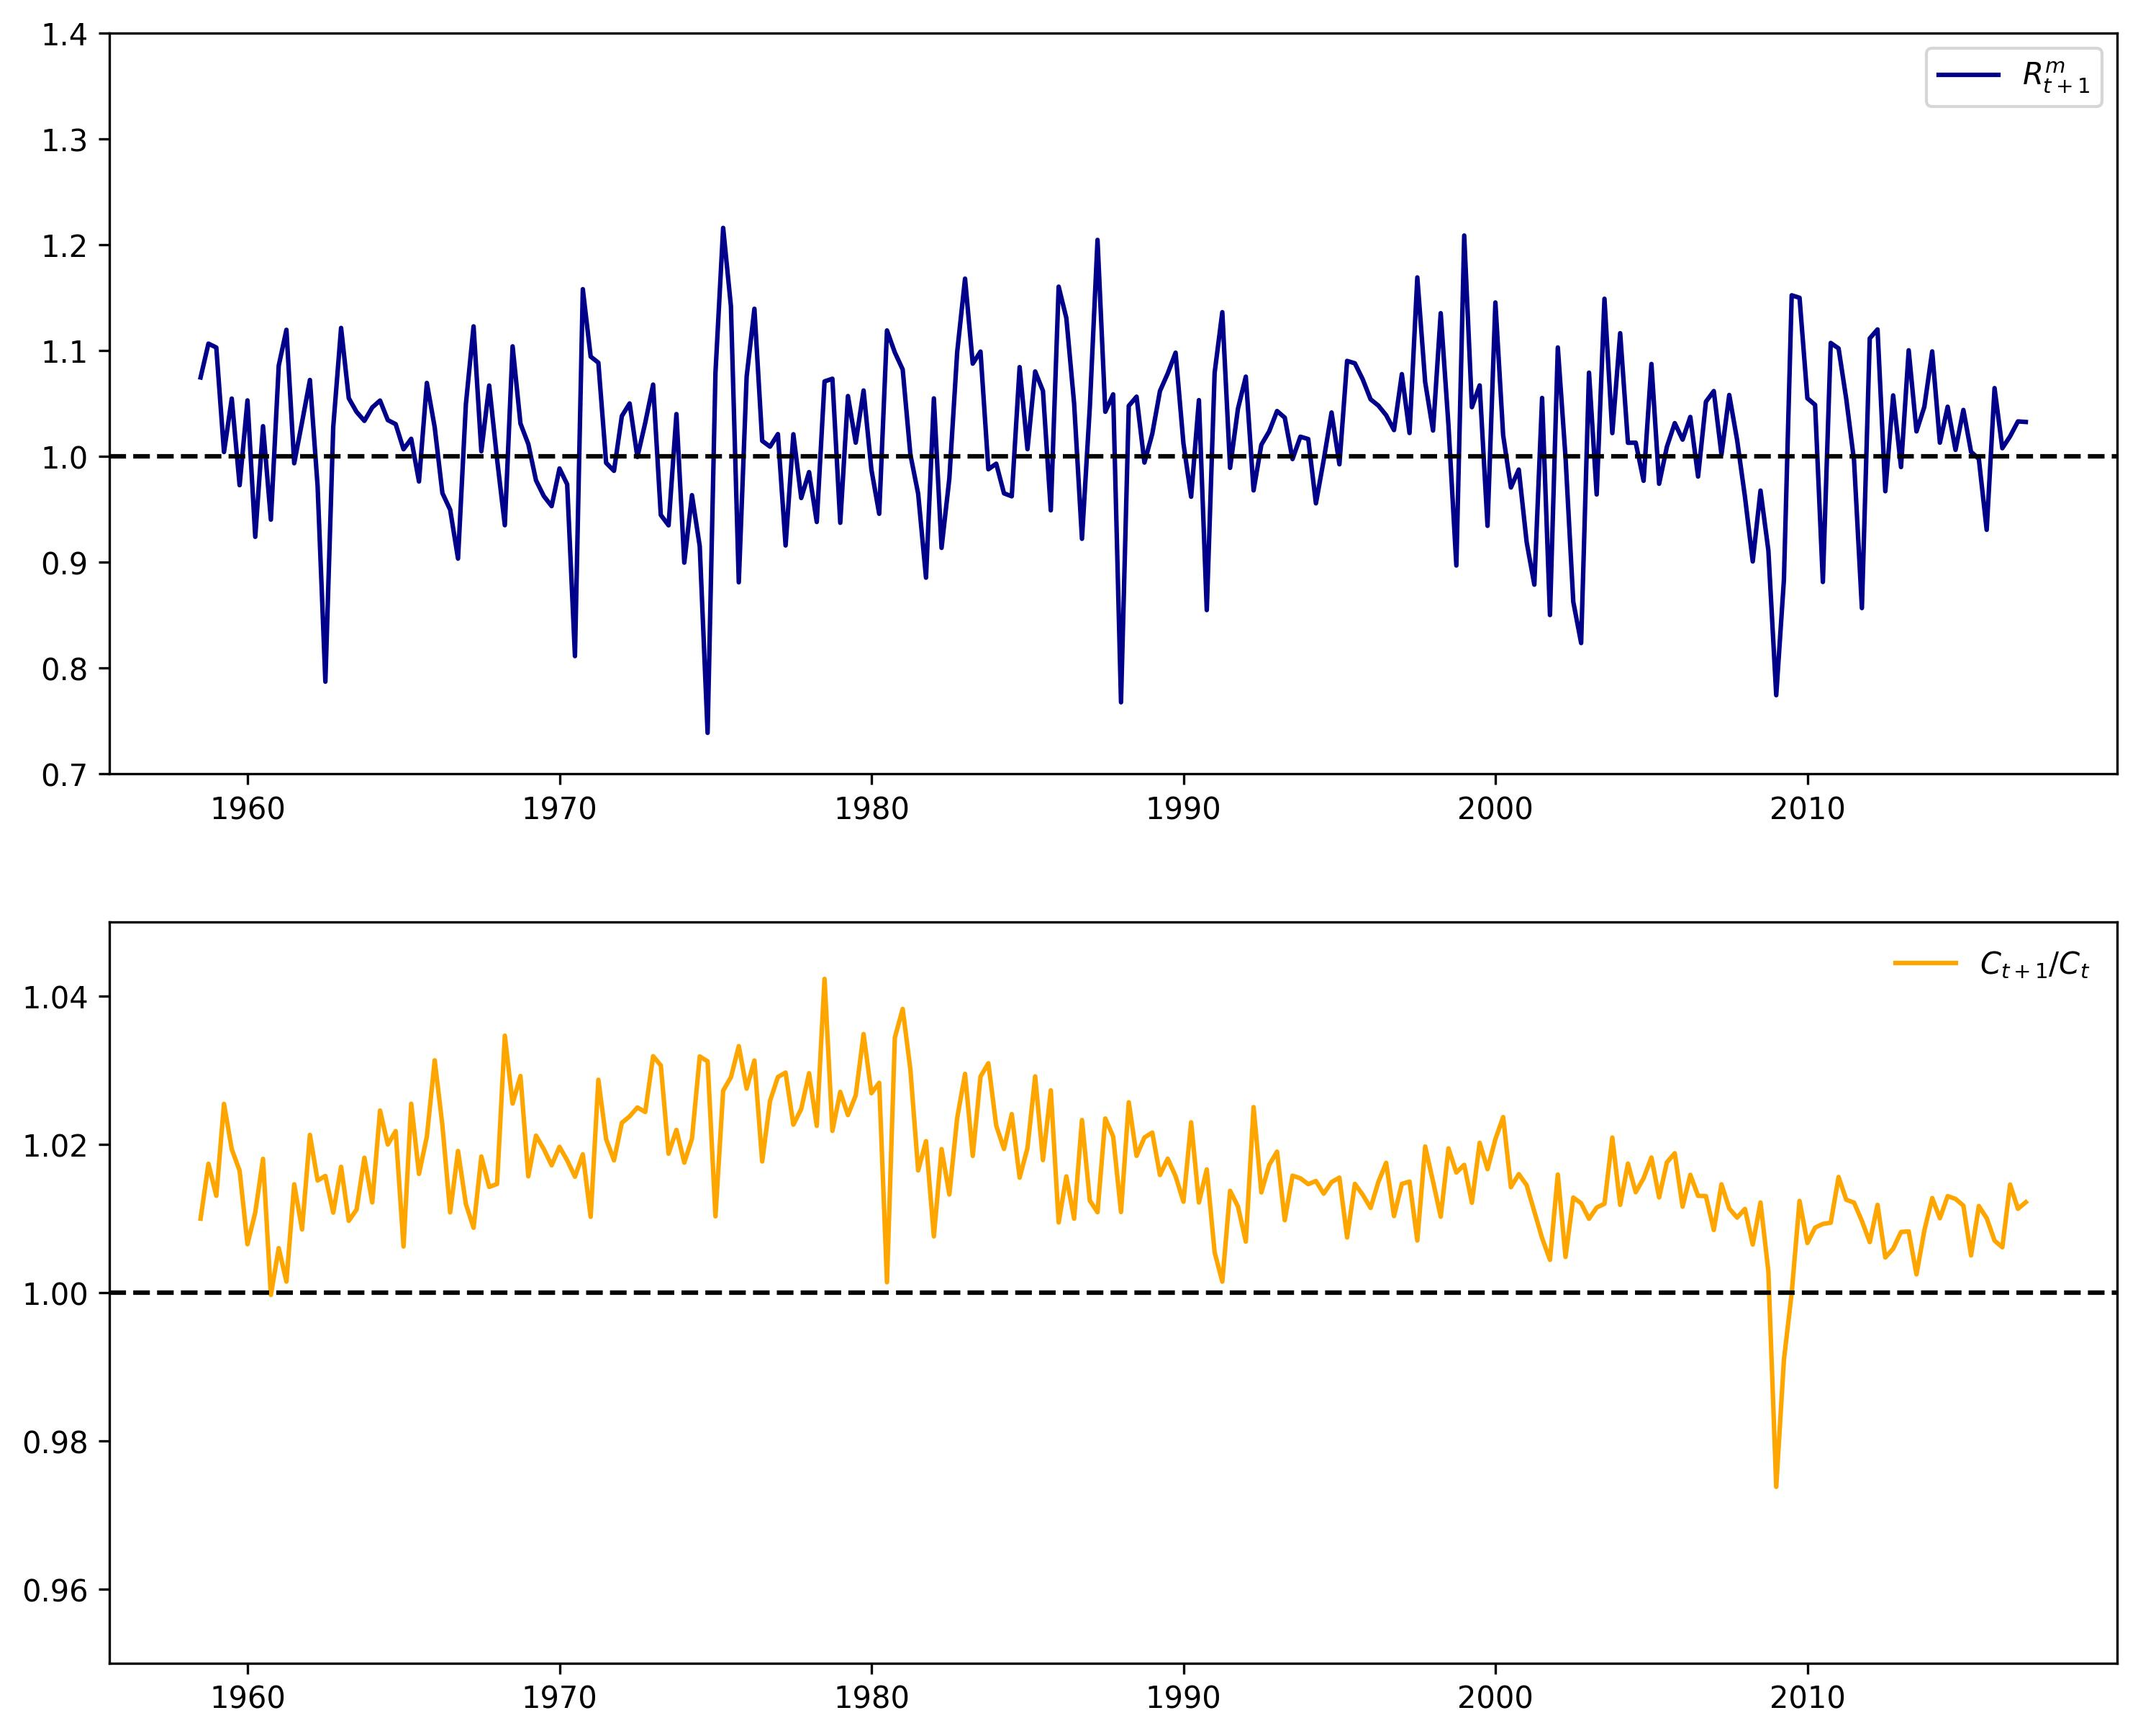
\includegraphics[width = .8\textwidth]{series.jpg}
        \caption{Series of \(R_t\) and \(C_t\) from 1958:Q1 to 2016:Q4}
        \label{fig:series}
    \end{figure}
    We start by defining some notation for this question. Following the lecture notes we denote 
    \[
        m\of{z_t, \theta} = m\of{\bp{R_{t+1}^m, C_t, C_{t+1}}, \bp{\beta, \gamma}} = R^m_{t+1}\beta\bp{\frac{C_{t+1}}{C_t}}^{-\gamma}-1
    \]
    and \(g_t\of\theta = T^{-1}\sum_t m\of{z_t, \theta}\) and \(\wh S_T\of\theta =T^{-1}\sum_t m\of{z_t,\theta}^2\). Therefore the J-criterion of the GMM estimator is given by
    \[
        J_T\of\theta = g_T\of\theta^\prime \wh S_T\of\theta^{-1} g_T\of\theta
    \]
    I then calculate the J-criterion for a grid of \(\gamma\) from 0 to 10 with length 1000. I used both the efficient weighting matrix (\(\wh S_T\)) and the identity matrix. The results are shown in Figure~\ref{fig:jcrit} and the optimal value of gamma seems to be close to 1 for both criteria.
    \begin{figure}[H]
        \centering
        \caption{J-criterion for the grid of \(\gamma\)}
        \label{fig:jcrit}
        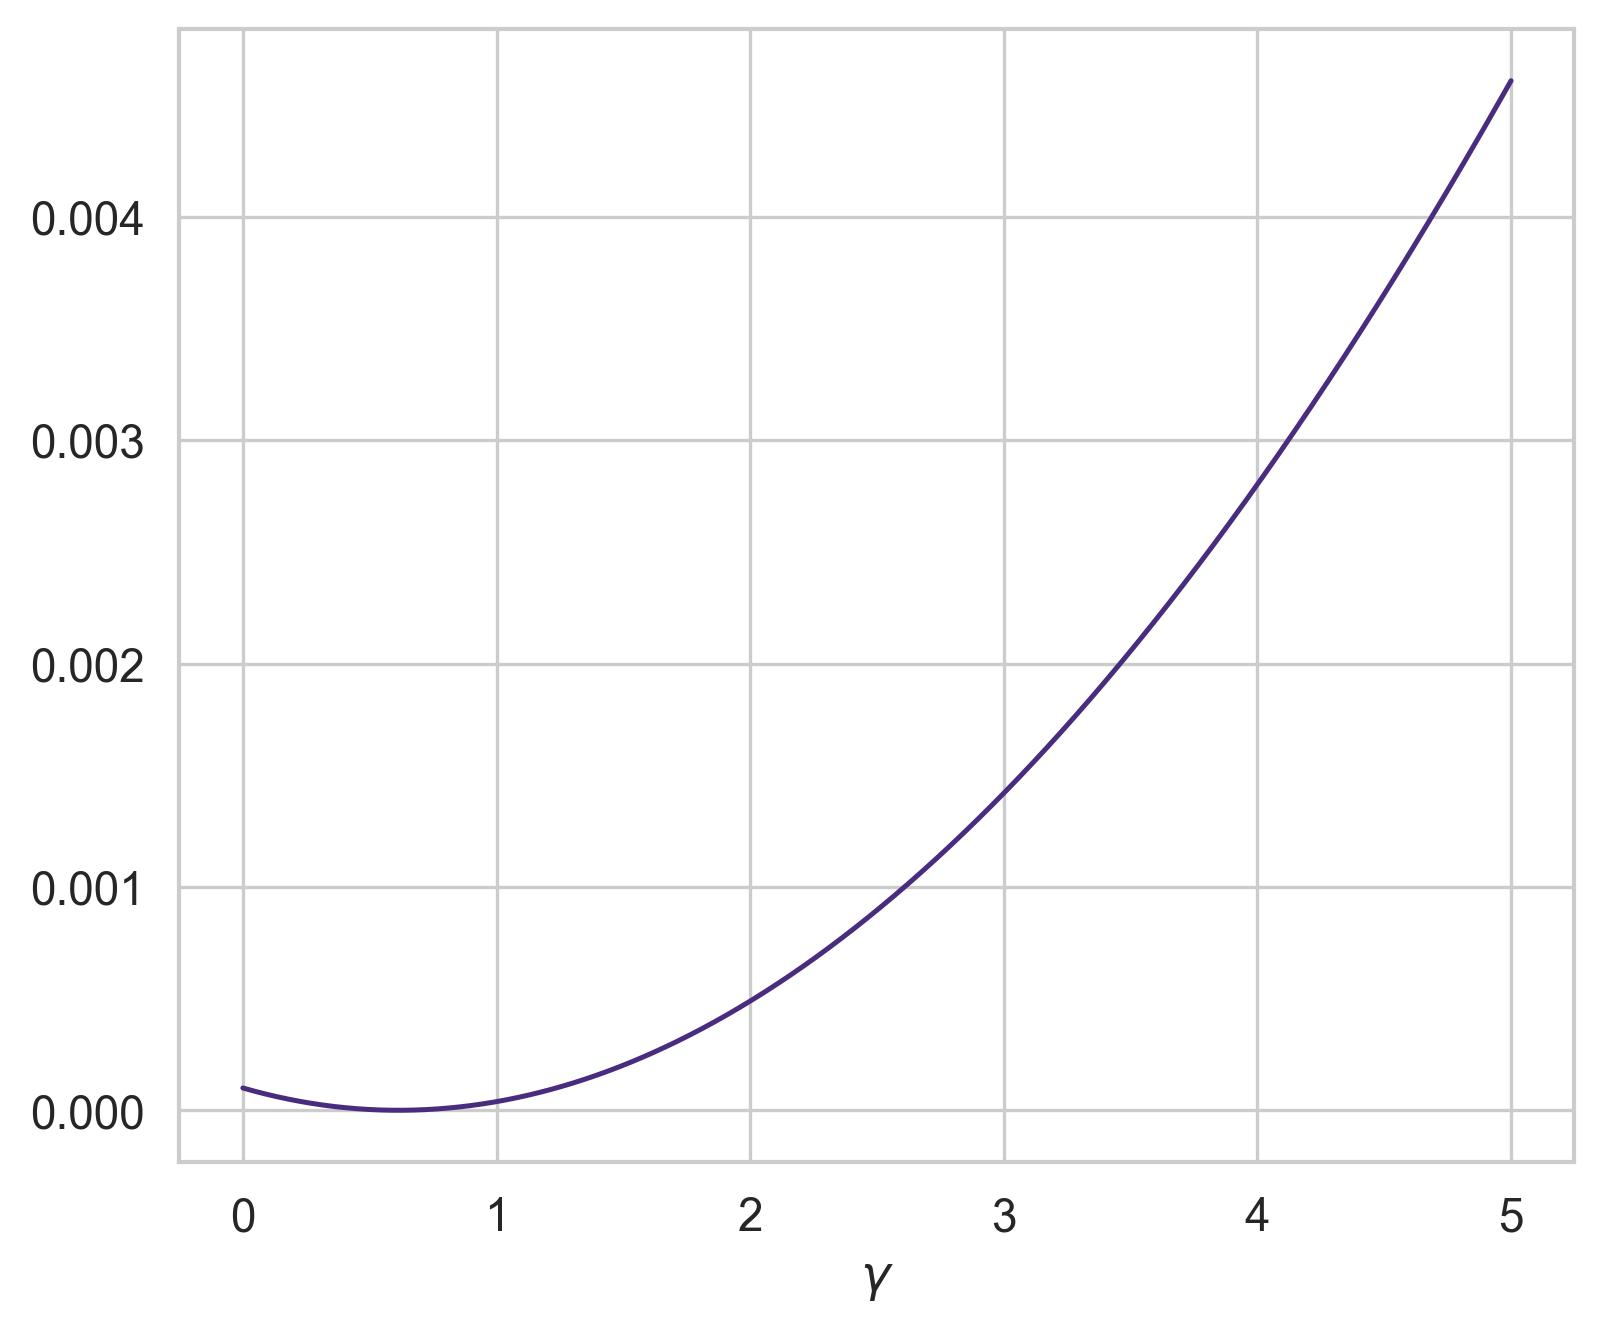
\includegraphics[width=0.6\textwidth]{jcrit.jpg}
    \end{figure}
    \item Using the conditional moment from Equation~\ref{eq:eq1}, we can use the instruments \(Z_t\) to write
    \[
        \E{m(z_t, \theta) Z_t} = 0
    \]
    so letting \(\wt m\of{z_t, \theta, Z_t} = m\of{z_t, \theta} Z_t\) we can rewrite the J-criterion and the efficient matrix as
    \begin{align*}
        \wt S_t\of\theta & = T^{-1} \sum_t \wt m\of{z_t, \theta, Z_t} \wt m\of{z_t, \theta, Z_t}^\prime = T^{-1} \sum_t m\of{z_t, \theta}^2 Z_t Z_T^\prime \\
        \wt J_T\of\theta & = g_T\of\theta^\prime \wt S_T\of\theta^{-1} g_T\of\theta
    \end{align*}
    I then calculate this criteria as in the previous question and display it in Figure~\ref{fig:jcrit_cond}. The results remain the same.
    \begin{figure}[H]
        \centering
        \caption{J-criterion for the grid of \(\gamma\) using the instruments \(Z_t\)}
        \label{fig:jcrit_cond}
        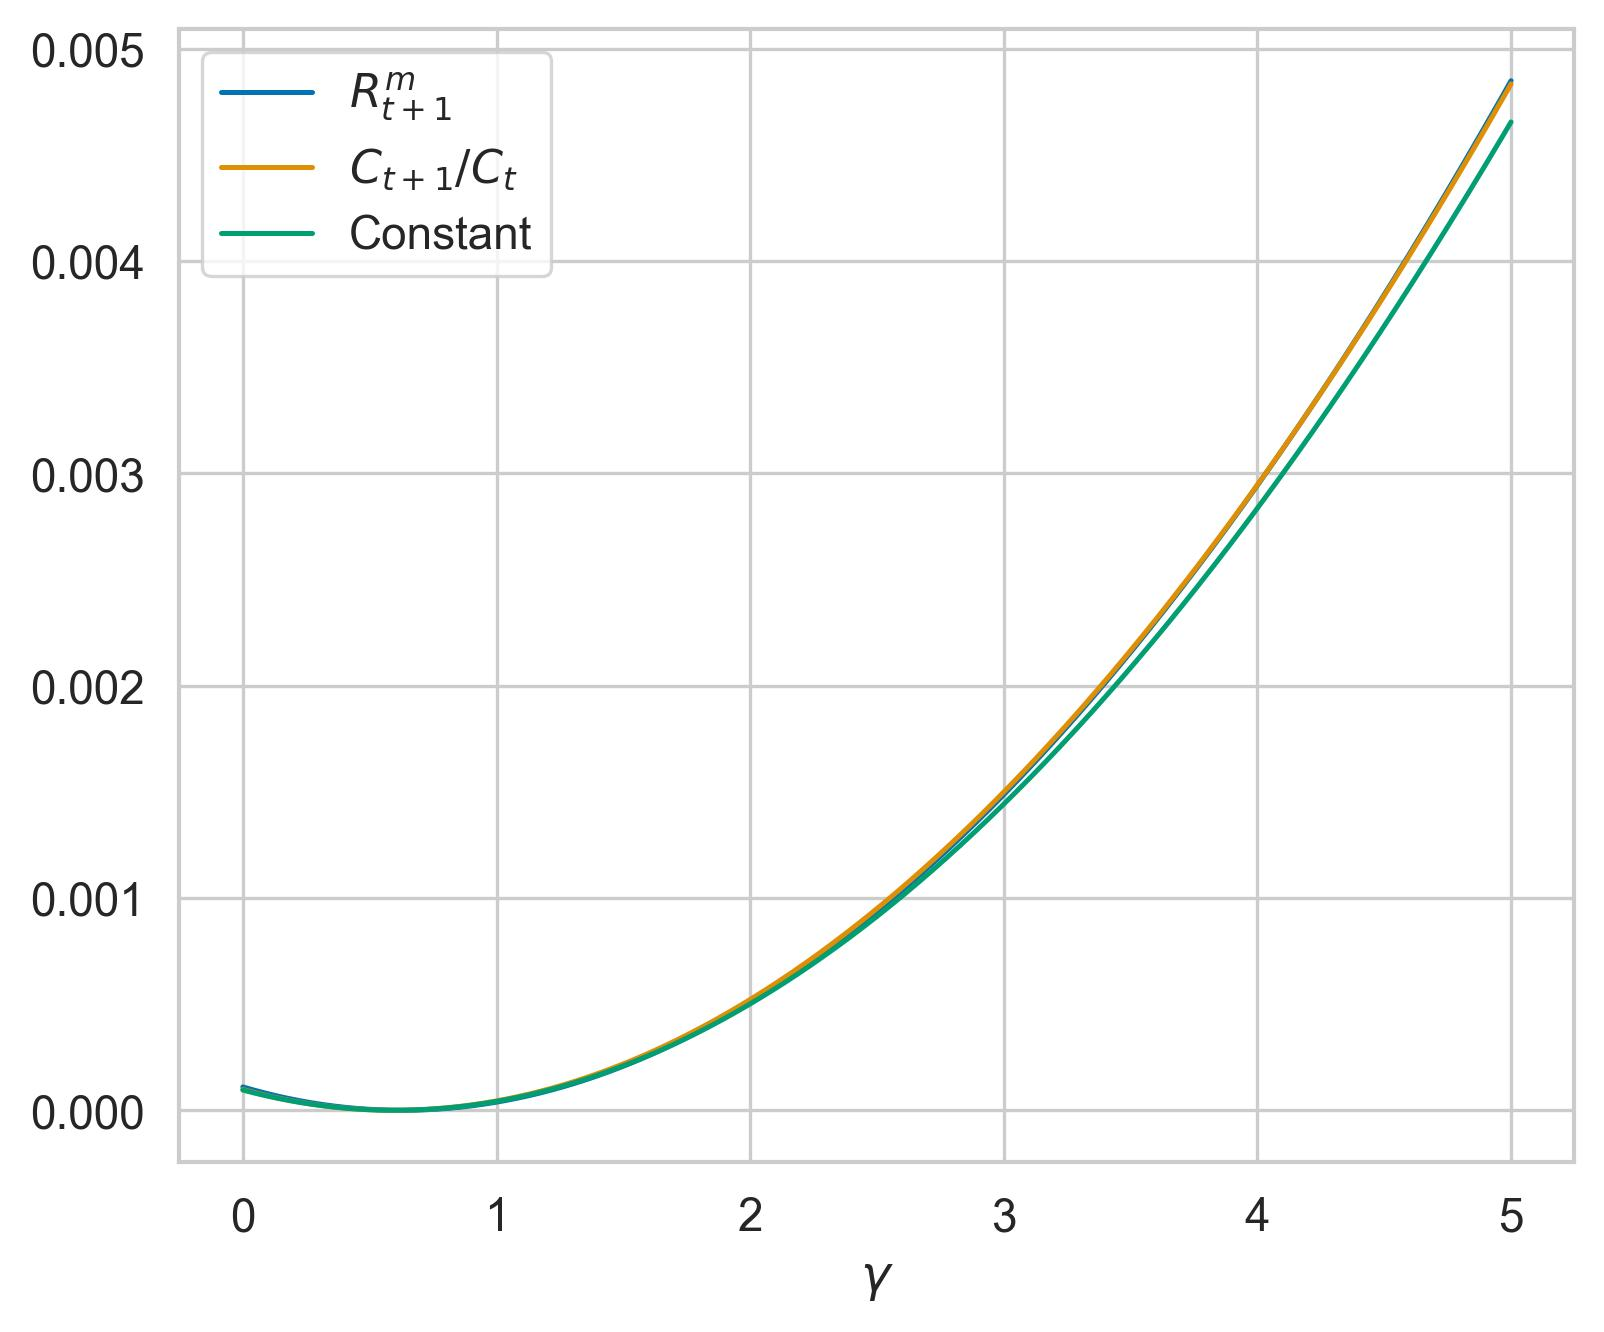
\includegraphics[width=0.6\textwidth]{jcrit_cond.jpg}
    \end{figure}

    \item I estimate the parameters using a the first lag of \(R_t\) and \(C_t\) as instruments as well as a constant. The model is estimated using the minimization of the moment conditions. For the minimization algorithm, I used as initial guess the value of \(\gamma\) that minimized the J-criterion in (a) with \(\beta = 0.99\). Since these parameters are restricted (\(\gamma > 0, \beta \in \bp{0,1}\)) I reparametrized the model to allow the algorithm to search over the entire real line which facilitates the minimization. Therefore the model is taken with
    \[
        \gamma = \frac{1}{1+\exp^{-\wt\gamma}} \hspace{25pt} \beta = \wt\beta^2
    \]
    Initially I tried to perform a two-step approach to estimate the parameters using the identity weighting matrix in the first step and using these estimates to calculate the efficient weighting matrix by calculating \(\widehat S(\beta,\gamma)\). This however did not turn out so well as the determinant of the estimated \(S\) was nearly zero, making the second-step estimate very volatile. I then kept the first stage as my final results which are reported below with the standard deviations in parenthesis:

    \begin{center}
        \begin{tabular}{ccccc}
$\beta$ = & 0.9900 & & $\gamma$ = & 0.6084 \\
& (0.0154) & & & (0.9286)
\end{tabular}
    \end{center}

    As we can see, the estimates of \(\gamma\) are close to the ones guessed on item (a) and \(\beta\) is really close to 0. We also note that the variance of \(\gamma\) is really high.

    To understand the stability of the estimates, I reestimate the model using a set of 10.000 random initial guesses and store the solutions for each one of them. The distribution of these solutions are shown in Figure~\ref{fig:solutions}. The results indicate that there may be two local solutions based on the modes of the marginal distribution in Figure~\ref{fig:solutions}. This presents a challenge to the estimation since it 

    \begin{figure}[H]
        \centering
        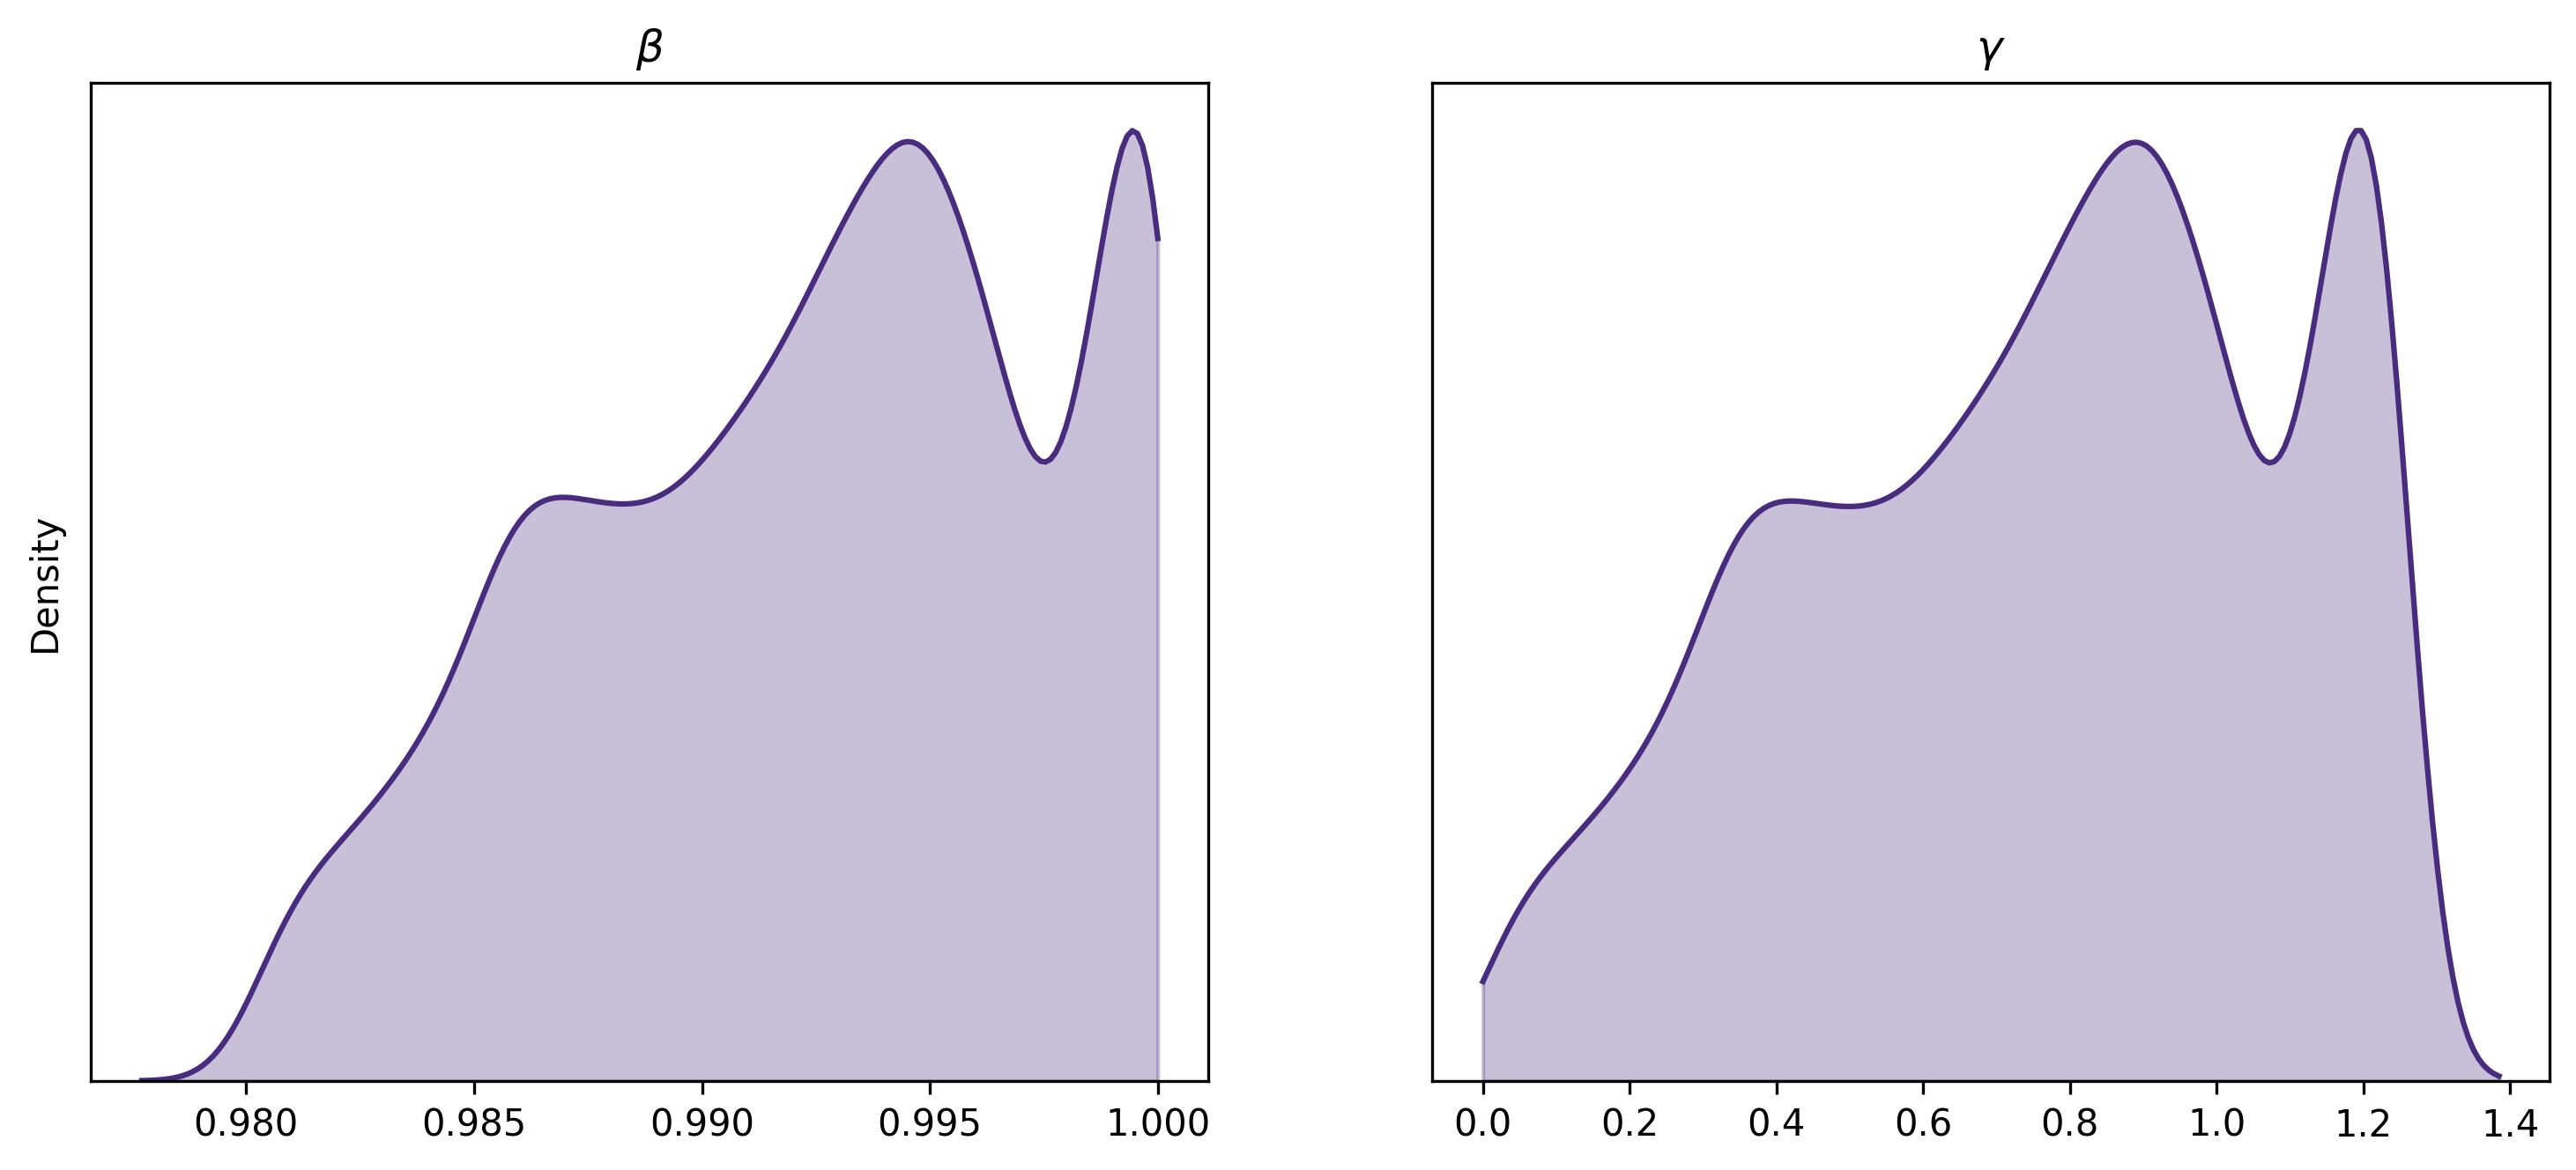
\includegraphics[width = \textwidth]{marg_solutions.jpg}
        \caption{Solutions for 10.000 random initial guesses}
        \label{fig:solutions}
    \end{figure}

    I now perform the Hausman test of overidentified restrictions whose null hypothesis is that a subset of the instruments is exogenous. If that is the case, then excluding (some) of the instruments would lead to a more efficient estimator. We analyze this by comparing the moment condition of both estimates. Under the null, a subset of the instruments can be used in a just-identified model to efficiently estimate the parameters. Under a just-identified model, the moment condition is perfectly matched and has zero average in the sample. Also, using the results of the previous problem set, we can compare an efficient and a consisent (but not efficient) estimator using the Hausman test. The test statistic is given by:
    \[
        \mathcal H = T \times \bs{\frac{1}{T}\sum_{t=1}^T m\bp{z_t, \wh\theta}}^\prime A \bs{\frac{1}{T}\sum_{t=1}^T m\of{z_t, \wh\theta}}
    \]
    The results are shown below:
    \begin{center}
        \begin{tabular}{ccccc} 
$\chi^2$ =& 4.5339 & & p-value =& 0.9668 
\end{tabular}
    \end{center}
    As we can see, the test is not able to reject the null so there may be exogenous instruments.


    \item I calculate the model using 1, 2, 3 and 4 lags of the instruments.    The  estimates are shown below:
    \begin{center}
        \begin{tabular}{@{\extracolsep{5pt}}lcccc} 
\\[-1.8ex]\hline 
\hline \\[-1.8ex] 
& \multicolumn{4}{c}{\textit{Number of Lags}} \\ 
& (1) & (2) & (3) & (4) \\ 
\hline \\[-1.8ex] 
$\beta$ & 0.990& 0.990& 0.990& 0.990\\ 
& (0.016)& (0.014)& (0.014)& (0.013)\\ 
$\gamma$ & 0.575& 0.566& 0.563& 0.563\\ 
& (0.941)& (0.835)& (0.846)& (0.806)\\ 
\hline \\[-1.8ex] 
N & 231 & 231 & 231 & 231\\ 
 $\mathcal H$ & 1.922 & 6.366 & 6.493 & 7.137\\ 
 p-value & 0.834 & 0.988 & 0.989 & 0.992 \\ 
\hline \hline \\[-1.8ex] 
\end{tabular}
    \end{center}
    The results are pretty similar all the set of instruments used and the interpretations of all the tests remain the same. We note that, as we increase the number of instruments, the estimation of \(\gamma\) gets more precise, judging by the decay in the standard deviations.
\end{enumerate}
\end{solution}